\documentclass{standalone}

\usepackage{graphicx}
\usepackage{tabularx,multirow,colortbl,booktabs}

\usepackage{tikz}
\usetikzlibrary{calc}
\usetikzlibrary{positioning}
\tikzset{
    between/.style args={#1 and #2}{
    	at = ($(#1)!0.5!(#2)$)
    }
}

\begin{document}

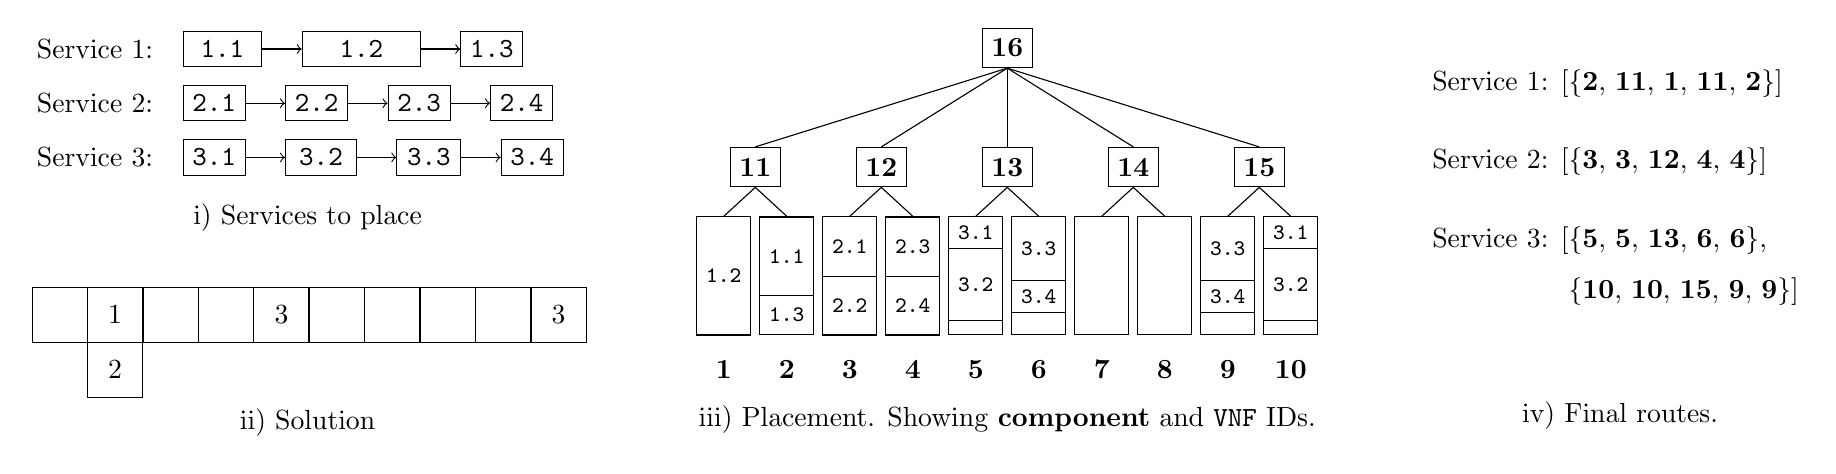
\begin{tikzpicture}[
        every node/.style={node distance=10mm and 1mm},
        server/.style={rectangle, draw=black, minimum width=.686cm},
        switch/.style={rectangle, draw=black, minimum size=.5cm},
        vnf/.style={rectangle, draw=black, minimum height = .4cm},
        solution/.style={draw, minimum size = .7cm},
    ]

    \def \vnfw {1};

    \node (S1) {Service 1:};
    \node[vnf] (S1V1) [right=.25cm of S1, minimum width = \vnfw cm] {\texttt{1.1}};
    \node[vnf] (S1V2) [right=.5cm of S1V1, minimum width = 1.5*\vnfw cm] {\texttt{1.2}};
    \node[vnf] (S1V3) [right=.5cm of S1V2, minimum width = 0.5*\vnfw cm] {\texttt{1.3}};

    \draw[->] (S1V1.east)  -- (S1V2.west);
    \draw[->] (S1V2.east)  -- (S1V3.west);

    \node (S2) [below=.2cm of S1] {Service 2:};
    \node[vnf] (S2V1) [right=.25cm of S2, minimum width = .75*\vnfw cm] {\texttt{2.1}};
    \node[vnf] (S2V2) [right=.5cm of S2V1, minimum width = .75*\vnfw cm] {\texttt{2.2}};
    \node[vnf] (S2V3) [right=.5cm of S2V2, minimum width = .75*\vnfw cm] {\texttt{2.3}};
    \node[vnf] (S2V4) [right=.5cm of S2V3, minimum width = .75*\vnfw cm] {\texttt{2.4}};

    \draw[->] (S2V1.east)  -- (S2V2.west);
    \draw[->] (S2V2.east)  -- (S2V3.west);
    \draw[->] (S2V3.east)  -- (S2V4.west);

    \node (S3) [below=.2cm of S2] {Service 3:};
    \node[vnf] (S3V1) [right=.25cm of S3, minimum width = .3*\vnfw cm] {\texttt{3.1}};
    \node[vnf] (S3V2) [right=.5cm of S3V1, minimum width = .9*\vnfw cm] {\texttt{3.2}};
    \node[vnf] (S3V3) [right=.5cm of S3V2, minimum width = .8\vnfw cm] {\texttt{3.3}};
    \node[vnf] (S3V4) [right=.5cm of S3V3, minimum width = .4\vnfw cm] {\texttt{3.4}};

    \draw[->] (S3V1.east)  -- (S3V2.west);
    \draw[->] (S3V2.east)  -- (S3V3.west);
    \draw[->] (S3V3.east)  -- (S3V4.west);

    \node (H1) [below=.4cm of S3] {};
    \node (C1) [right=1cm of H1] {i) Services to place};

    \node (H2) [left=.2cm of H1] {};
    \node (BL1) [below=-.5cm of H2] {};

    \node[solution] (SL1) [below=of BL1] {};
    \node[solution] (SL2) [right=-0.01cm of SL1] {1};
    \node[solution] (SL2B) [below=-0.015cm of SL2] {2};

    \node[solution] (SL3) [right=-0.01cm of SL2] {};
    \node[solution] (SL4) [right=-0.01cm of SL3] {};
    \node[solution] (SL5) [right=-0.01cm of SL4] {3};
    \node[solution] (SL6) [right=-0.01cm of SL5] {};
    \node[solution] (SL7) [right=-0.01cm of SL6] {};
    \node[solution] (SL8) [right=-0.01cm of SL7] {};
    \node[solution] (SL9) [right=-0.01cm of SL8] {};
    \node[solution] (SL10) [right=-0.01cm of SL9] {3};

    \node (H2) [below=1cm of SL1] {};
    \node (C2) [below=2cm of C1] {ii) Solution};

    \node (BL2) [right=7cm of S1] {};

    \node[server]      (S1)        [below=2cm of BL2, minimum height = 1.5cm] {};
    \node[server]      (S2)        [right=of S1, minimum height = 1.5cm]  {};
    \node[server]      (S3)        [right=of S2, minimum height = 1.5cm]  {};
    \node[server]      (S4)        [right=of S3, minimum height = 1.5cm]  {};
    \node[server]      (S5)        [right=of S4, minimum height = 1.5cm]  {};
    \node[server]      (S6)        [right=of S5, minimum height = 1.5cm]  {};
    \node[server]      (S7)        [right=of S6, minimum height = 1.5cm]  {};
    \node[server]      (S8)        [right=of S7, minimum height = 1.5cm]  {};
    \node[server]      (S9)        [right=of S8, minimum height = 1.5cm]  {};
    \node[server]      (S10)       [right=of S9, minimum height = 1.5cm]  {};

    \node () [below=0.2cm of S1] {\textbf{1}};
    \node () [below=0.2cm of S2] {\textbf{2}};
    \node () [below=0.2cm of S3] {\textbf{3}};
    \node () [below=0.2cm of S4] {\textbf{4}};
    \node () [below=0.2cm of S5] {\textbf{5}};
    \node () [below=0.2cm of S6] {\textbf{6}};
    \node () [below=0.2cm of S7] {\textbf{7}};
    \node () [below=0.2cm of S8] {\textbf{8}};
    \node () [below=0.2cm of S9] {\textbf{9}};
    \node () [below=0.2cm of S10] {\textbf{10}};

    \node[] (VNF11) [above=-1.018 cm of S2, draw, minimum width = .5cm, minimum height = \vnfw cm] {\footnotesize \texttt{1.1}};
    \node[] (VNF12) [above=-1.52 cm of S1, draw, minimum width = .5cm, minimum height = 1.5\vnfw cm] {\footnotesize \texttt{1.2}};
    \node[] (VNF13) [above=-1.508 cm of S2, draw, minimum width = .5cm, minimum height = .49\vnfw cm] {\footnotesize \texttt{1.3}};

    \node[] (VNF21) [above=-.77 cm of S3, draw, minimum width = .5cm, minimum height = .755*\vnfw cm] {\footnotesize \texttt{2.1}};
    \node[] (VNF22) [above=-1.52 cm of S3, draw, minimum width = .5cm, minimum height = .75\vnfw cm] {\footnotesize \texttt{2.2}};
    \node[] (VNF23) [above=-.77 cm of S4, draw, minimum width = .5cm, minimum height = .75\vnfw cm] {\footnotesize \texttt{2.3}};
    \node[] (VNF24) [above=-1.52 cm of S4, draw, minimum width = .5cm, minimum height = .75\vnfw cm] {\footnotesize \texttt{2.4}};

    \node[] (VNF31) [above=-0.42 cm of S5, draw, minimum width = .5cm, minimum height = .3\vnfw cm] {\footnotesize \texttt{3.1}};
    \node[] (VNF32) [above=-1.33 cm of S5, draw, minimum width = .5cm, minimum height = .9\vnfw cm] {\footnotesize \texttt{3.2}};
    \node[] (VNF33) [above=-0.82 cm of S6, draw, minimum width = .5cm, minimum height = .8\vnfw cm] {\footnotesize \texttt{3.3}};
    \node[] (VNF33) [above=-1.23 cm of S6, draw, minimum width = .5cm, minimum height = .4\vnfw cm] {\footnotesize \texttt{3.4}};

    \node[] (VNF31B) [above=-0.42 cm of S10, draw, minimum width = .5cm, minimum height = .3\vnfw cm] {\footnotesize \texttt{3.1}};
    \node[] (VNF32B) [above=-1.33 cm of S10, draw, minimum width = .5cm, minimum height = .9\vnfw cm] {\footnotesize \texttt{3.2}};
    \node[] (VNF33B) [above=-0.82 cm of S9, draw, minimum width = .5cm, minimum height = .8\vnfw cm] {\footnotesize \texttt{3.3}};
    \node[] (VNF33B) [above=-1.23 cm of S9, draw, minimum width = .5cm, minimum height = .4\vnfw cm] {\footnotesize \texttt{3.4}};

    \node[] 		 (H1) 		 [between=S1 and S2] {};
    \node[] 		 (H2) 		 [between=S3 and S4] {};
    \node[] 		 (H3) 		 [between=S5 and S6] {};
    \node[] 		 (H4) 		 [between=S7 and S8] {};
    \node[] 		 (H5) 		 [between=S9 and S10] {};

    \node[switch]      (E1)        [above = of H1] {\textbf{11}};
    \node[switch]      (E2)        [above = of H2] {\textbf{12}};
    \node[switch]      (E3)        [above = of H3] {\textbf{13}};
    \node[switch]      (E4)        [above = of H4] {\textbf{14}};
    \node[switch]      (E5)        [above = of H5] {\textbf{15}};

    \node[switch]      (M1)        [above = of E3] {\textbf{16}};

    \draw[-] (S1.north)  -- (E1.south);
    \draw[-] (S2.north)  -- (E1.south);
    \draw[-] (S3.north)  -- (E2.south);
    \draw[-] (S4.north)  -- (E2.south);
    \draw[-] (S5.north)  -- (E3.south);
    \draw[-] (S6.north)  -- (E3.south);
    \draw[-] (S7.north)  -- (E4.south);
    \draw[-] (S8.north)  -- (E4.south);
    \draw[-] (S9.north)  -- (E5.south);
    \draw[-] (S10.north)  -- (E5.south);

    \draw[-] (E1.north)  -- (M1.south);
    \draw[-] (E2.north)  -- (M1.south);
    \draw[-] (E3.north)  -- (M1.south);
    \draw[-] (E4.north)  -- (M1.south);
    \draw[-] (E5.north)  -- (M1.south);

    \node (CR) [below=1.4cm of H3] {iii) Placement. Showing \textbf{component} and \texttt{VNF} IDs.};

    \node (BL3) [right=4.7cm of M1] {};

    \node (H1) [below=0.2cm of BL3] {};
    \node (H2) [below=0.75cm of H1] {};
    \node (H3) [below=0.75cm of H2] {};
    \node (H4) [below=0.4cm of H3] {};

    \node (T1) [right=0cm of H1] {Service 1: [\{\textbf{2}, \textbf{11}, \textbf{1}, \textbf{11}, \textbf{2}\}]}; 
    \node (T2) [right=0cm of H2] {Service 2: [\{\textbf{3}, \textbf{3}, \textbf{12}, \textbf{4}, \textbf{4}\}]};
    \node (T2) [right=0cm of H3] {Service 3: [\{\textbf{5}, \textbf{5}, \textbf{13}, \textbf{6}, \textbf{6}\},};
    \node (T2) [right=1.73cm of H4] {\{\textbf{10}, \textbf{10}, \textbf{15}, \textbf{9}, \textbf{9}\}]};

    \node (H4) [below=1.15cm of T2] {};
    \node (CR) [right=-2.3cm of H4] {iv) Final routes.};

\end{tikzpicture}

\end{document}